
\documentclass[12pt,a4paper]{article} % Use A4 paper with a 12pt font size - different paper sizes will require manual recalculation of page margins and border positions

% Generated with LaTeXDraw 2.0.8
% Mon Jun 17 19:00:40 EDT 2013
\usepackage[usenames,dvipsnames]{pstricks}
\usepackage{epsfig}
\usepackage{pst-grad} % For gradients
\usepackage{pst-plot} % For axes
%\usepackage{marginnote} % Required for margin notes
%\usepackage{wallpaper} % Required to set each page to have a background
%\usepackage{lastpage} % Required to print the total number of pages
\usepackage[left=1.3cm,right=4.6cm,top=1.8cm,bottom=4.0cm,marginparwidth=3.4cm]{geometry} % Adjust page margins
\usepackage{amsmath} % Required for equation customization
\usepackage{amssymb} % Required to include mathematical symbols
\usepackage{xcolor} % Required to specify colors by name
\usepackage{amsthm}
\usepackage{float}


\setlength{\parindent}{0cm} % Remove paragraph indentation
\newcommand{\tab}{\hspace*{2em}} % Defines a new command for some horizontal space


\title{Calculus Review - Preliminaries}
%----------------------------------------------------------------------------------------

\newtheorem{defn}{Definition}
\newtheorem{example}{Example}
\newtheorem{prop}{Proposition}
\newtheorem{exer}{Exercises}
\newtheorem{thm}{Therorem}
\begin{document}
\maketitle
\section{Preliminaries}
\subsection{Absolute Value}
Many students who have taken Calculus courses aren't aware that the term 'calculus' simply means 'a method of calculation'. What we have become to call Calculus (with a capital 'C') is actually shortened from 'Calculus of Limits'. Everything we do in Calculus concerns limits. We begin with limits of functions at a point, at infinity, etc. and then study derivatives, which are limits of slopes. Integrals are limits of sums. Sums of infinite series are defined as limits of sequences of partial sums.\\

Because everything we review will concern limits, it's pretty important to understand what limits are. Most students will recall that\\

$$\lim\limits_{x\rightarrow a} f(x) = L$$

means that 'as $x$ gets close to $a$, $f(x)$ gets close to $L$'. This is a great intuitive statement, but we need to be more precise, starting with what 'close' means.\\

It is helpful to think of such things as $|x -a|$ as 'distances'.  So, when you see the absolute value of a difference, you really should be thinking of the distance between the numbers on the real line.  For example, consider:
$$|(-2) - 1|$$
We can think of this expression as the distance between $-2$ and $1$ on the number line:\\
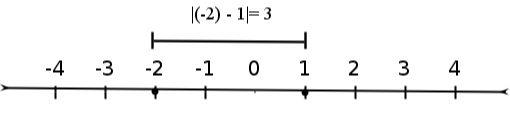
\includegraphics[]{dist.jpg}

Thus, we can interpret $x$ is close to $a$ to mean that $|x-a|$ is small (and similar for $f(x)$ and $L$ - they are close when $|f(x) - L|$ is small).\\

Our job in the next lesson will be to make it clear what 'small' means, but for now, here are some helpful properties of absolute value:\\

\begin{enumerate}
\item If $|x|\leq a$, then $-a\leq x\leq a$
\item Triangle inequality:  $|x +y| \leq |x| +|y|$
\item Reverse triangle inequality: $||x|-|y|| \leq |x-y|$
\end{enumerate}

\subsection{Functions}
Recall that a function is a rule that assigns an output value to some input value.  For example, a rule might be to take the input (a real number) and output its square (also a real number).  We can call this rule $f$ and write:
\begin{equation*}
f(x) = x^2
\end{equation*}
Mathematicians like to be clear on the input (domain) of a function and the output (range) of a function.  Because our $f$ above can take any real number and will output a real number, we say that $f$ is a real-valued function of a real variable.  That is a lot to say.  We can use a shorthand, by denoting the set of real numbers by $\mathbb{R}$.  We then write:
\begin{equation}
f:\mathbb{R}\rightarrow \mathbb{R}
\end{equation}
This says the same thing as '$f$ is a real-valued function of a real variable', but it is shorter, and we may read it as '$f$ is a function from $\mathbb{R}$ to $\mathbb{R}$'.  You will encounter functions on other sets, for example, $\mathbb{N}$ - the natural numbers, $\mathbb{Z}$ - the integers, etc.  We will mostly focus on real functions of real variables for the purposes of these notes. 

\end{document}